%\documentclass[handout]{beamer}
\documentclass[ignorenonframetext]{beamer}
\usepackage{textpos}
\usepackage{graphicx}
\usepackage{pgf}
\usepackage{caption}
\usepackage{listings}
\usepackage{multimedia}
\usepackage{gensymb}
\usepackage{amsmath, mathrsfs}

% \captionsetup[figure]{labelformat=empty}% redefines the caption setup of the figures environment in the beamer class.

\usetheme{Boadilla}
\usefonttheme{serif}
% \mode<presentation>
% {
%  \usefonttheme{serif}
% % \useoutertheme{sidebar}
% %   \logo{\includegraphics[height=1cm]{elec_logo.pdf}}
% }

\title[TART Imaging]{Imaging with TART Part 1: Getting the tools}

\author[Molteno]{Tim Molteno}

\institute[Otago]
{
  Electronics Research Foundation (NZ) \\
  and \\
  Department of Physics\\
  University of Otago \\
  Dunedin, New Zealand.\\
  tim@elec.ac.nz\\
  \vspace{2cm}
  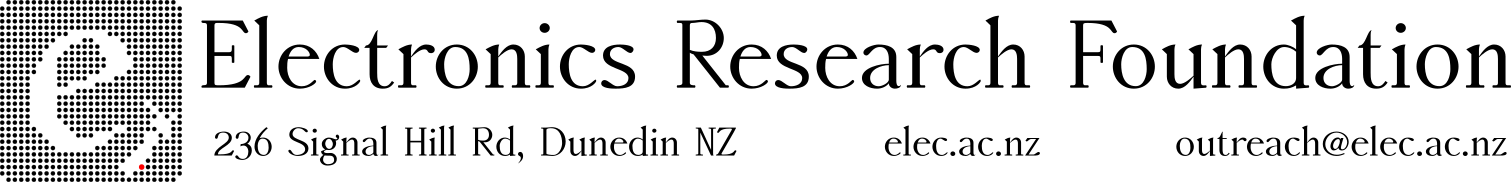
\includegraphics[width=0.7\linewidth]{../tart_overview/fig/elec_header_font.pdf}
}

% \titlegraphic{\includegraphics[width=2cm]{fig/elec_logo.pdf}\hspace*{4.75cm}~%
%    \includegraphics[width=2cm]{fig/elec_logo.pdf}
% }

\logo{\pgfputat{\pgfxy(-0.72,7.7)}{\pgfbox[center,base]{\includegraphics[width=1cm]{../tart_overview/fig/elec_logo.pdf}}}}

\date[UWC 06/2024] % (optional, should be abbreviation of conference name)
{}

% \addtobeamertemplate{headline}{}{%
% \begin{textblock*}{100mm}(0.87\textwidth,2mm)
% \includegraphics[height=1.5cm]{elec_logo.pdf}
% \end{textblock*}}

\begin{document}

% Abstract: In this talk I'll give an overview of Africa's newest radio telescope, the TART, recently installed in Mauritius in a joint effort between SARAO, the University of Otago (NZ). I'll talk about TARTs origins, it's design and open-source philosophy as well as the upcoming project to install TART telescopes in the SKA African partner nations. I'll also include some details about improvements that will appear in TART-3, the next version of TART!

\begin{frame}
  \titlepage
\end{frame}
 
\begin{frame}
\vspace{1cm}

  \includegraphics[width=\linewidth]{../tart_overview/fig/spiral.jpeg}\\
  \centering{A TART radio telescope under construction in Mauritius}
\end{frame}


\begin{frame}
  \tableofcontents
  % You might wish to add the option [pausesections]
\end{frame}

% \section{Origins of TART}

\begin{frame}[fragile]{TART Tools}
%    \includegraphics[width=\linewidth]{fig/albatross_frame.png}
  The TART software for imaging run in an environment called \href{https://github.com/caracal-pipeline/stimela}{stimela}. This is the software framework for the worlds largest radio telescopes.

  \begin{block}{Install}
  \begin{verbatim}
   pip install tart-tools
  \end{verbatim}
  \end{block}

  Notes:
  \begin{itemize}
   \item Should work on Linux and windows (WSL2).
   \item On a mac? Run a linux virtual machine.
  \end{itemize}
   \begin{block}{Homework}
   Please do this right away, and run a test script (see later), so we can use it tomorrow.
   \end{block}

\end{frame}


\begin{frame}[fragile]{Sample Imaging Recipe}
There is a sample recipe that should also be run:
\begin{itemize}
 \item Download it from \url{https://github.com/tart-telescope/tart_cargo}
 \item In test/example-recipe.yml.
\end{itemize}
\begin{block}{Run It}
 \begin{verbatim}
  stimela run example_recipe.yml tart=tart-kenya
 \end{verbatim}
\end{block}
 The first time this is run, it will take a long time and download a large docker image. Roughly 1 GB!
\end{frame}

\begin{frame}{Output}
\begin{columns}
 \begin{column}{0.7\linewidth}
\includegraphics[width=\linewidth]{images/obs_00000.hdf.png}
 \end{column}
 \begin{column}{0.3\linewidth}
 \begin{itemize}
  \item Known sources circled.
  \item Round!
 \end{itemize}
 \end{column}
\end{columns}
\end{frame}


\begin{frame}[fragile]{CASA Tools}
%    \includegraphics[width=\linewidth]{fig/albatross_frame.png}
  \href{https://github.com/caracal-pipeline/cult-cargo}{Cult-Cargo} is a suite of tools written by the radio astronomy community. Useful for making square images.

  \begin{block}{Install}
  \begin{verbatim}
   pip install cult-cargo
  \end{verbatim}
  \end{block}

  Notes:
  \begin{itemize}
   \item Should work on Linux and windows (WSL2).
   \item On Apple hardware, run a linux virtual machine.
  \end{itemize}
   \begin{block}{Homework}
   Download the test data from the google drive, and the script called 'full-tart-imaging.yml'
  \begin{verbatim}
   stimela run full-tart-imaging.yml
  \end{verbatim}

   \end{block}

\end{frame}

\section{What is going on behind the scenes}

\frame{\tableofcontents[currentsection]}


\begin{frame}
 \includegraphics[width=\linewidth]{../tart_overview/fig/browser_view.png}
\end{frame}

\begin{frame}[containsverbatim]
\frametitle{TART API: Access data from anywhere}
TART data and control are done throught a web-based API. 

\centering{\url{https://api.elec.ac.nz/tart/bw-biust/}}

\begin{lstlisting}[language=Python, frame=single, basicstyle=\footnotesize]
 import requests
 
 api_endpoint = "https://api.elec.ac.nz/tart/bw-biust/api/"
 r = requests.get(api_endpoint + "/v1/imaging/vis")
 print(r.json())
\end{lstlisting}

\end{frame}

% \begin{frame}{Synthesis Imaging}
% Measure complex visibility $V_{ij}$ by correlating signals from antenna $i$ and $j$.
% \[ V_{ij} = \frac{1}{T} \int_0^T E_i(t) E_j^{\star}(t) dt \]
% \begin{columns}
%  \begin{column}{0.55\linewidth}
% \begin{enumerate}
%  \item 276 Pairs of antennas
%  \item 16.368 MHz sampling rate per antenna
%  \item Real-time correlation in FPGA
%  \item 4.5 Giga MAC per second
%  \item T $\sim$ 1 second
% \end{enumerate}
%  \end{column}
%  \begin{column}{0.45\linewidth}
%  \includegraphics[width=\linewidth]{fig/papilio_pro.jpg}
%  \end{column}
% \end{columns}
% 
% \end{frame}
% 
% \begin{frame}{Synthesis Continued...}
% Fourier transform relationship between radio sky brightness $I(l,m)$ and
% visibility $V(u,v)$,
% \[
%   V(u,v) = \int I(l,m) e^{2\pi j(lu  + mv)} dl dm
% \]
% Obtain $I(l,m)$ through inverse Fourier transform of $V(u,v)$, 
% \[
%  I(l,m) = \mathscr{F}^{-1}\{V(u,v)\}
% \]
% where $V(u,v)$ is the visibility function sampled in the $uv$-plane at the locations of each antenna $(u_{ij},v_{ij})$ pair. 
% \end{frame}
% 

% \section{Expected \& Unexpected Results}


\begin{frame}{What the future holds}
 \begin{columns}
  \begin{column}{0.6\linewidth}
    \begin{itemize}
    \item TART 4.0?
    \item Transient event detection
    \item More workshops! Bangaladesh, Morrocco, Malta, Berkeley
    \item Automatic tracking of space Debris
    \item New Array Designs
    \item New imaging algorithms (Gridless, Direct from Data)
    \end{itemize}
  \end{column}
  \begin{column}{0.4\linewidth}
    \includegraphics[width=\linewidth]{../tart_overview/fig/tart3.jpg}
  \end{column}
\end{columns}
    \pause
    \begin{block}{}
     \begin{center} Questions? \end{center}
    \end{block}

\end{frame}



\end{document}
